\chapter{METODOLOGIA}

Metodologia e os materiais serão descritos neste capítulo


\section{LEGENDA}


\begin{description}[leftmargin=*, widest=FP]
    \item[\textbf{TP} (True Positive):] Verdadeiro Positivo. Representa o número de instâncias em que o modelo previu corretamente a classe positiva.
    \item[\textbf{TN} (True Negative):] Verdadeiro Negativo. Indica a quantidade de instâncias em que o modelo previu corretamente a classe negativa.
\end{description} 



\section{CRONOGRAMA DE ATIVIDADES}

\begin{figure}[htbp]
    \centering
    \caption{Cronograma de atividades do semestre (Agosto -- Dezembro).}
    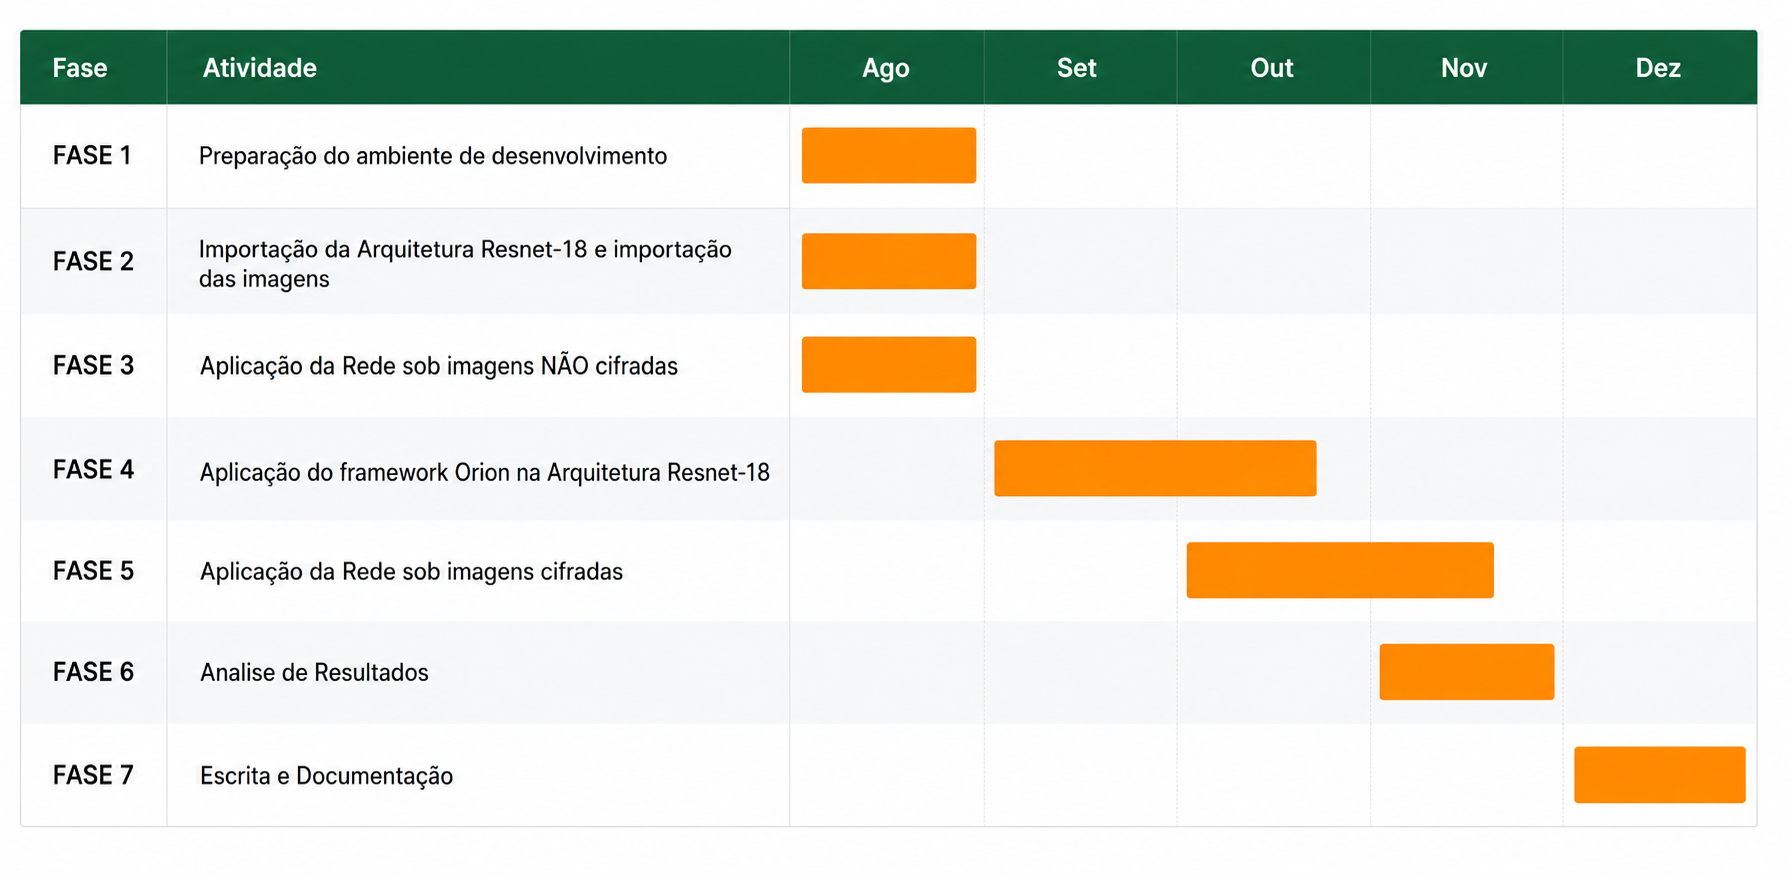
\includegraphics[width=1.0\textwidth]{imagens/cronograma-atv.png}
    \label{fig:cronograma-agosto-dezembro}
    
\end{figure}